% Chapter 1

\chapter{Introduction} % Main chapter title

\label{Chapter1} % For referencing the chapter elsewhere, use \ref{Chapter1} 

\lhead{Chapter 1. \emph{ Introduction }} % This is for the header on each page - perhaps a shortened title

%----------------------------------------------------------------------------------------
\section{Overview}
Healthcare sector is totally different from other industry. It is on high priority sector and people expect highest level of care and services regardless of cost. After the success of deep learning in other real-world application, it is also providing exciting solutions with good accuracy for medical imaging and is a key method for future applications in health sector. Brain is an organ that controls activities of all the parts of the body. Recognition of automated brain tumor in
Magnetic resonance imaging (MRI) is a difficult task due to complexity of size and location variability. In this thesis, statistical analysis morphological and thresholding techniques are proposed to process the images obtained by MRI for Tumor Detection from Brain MRI Images. 

In recent times, the introduction of information technology and e-health care system in the medical field helps clinical experts to provide effective diagnosis, treatment and monitoring of the disease for better health care to the patient.The most recent big advances in Magnetic Resonance Imaging (MRI) technology have been on the software side, enabling faster contrast scans. Magnetic resonance imaging (MRI) is a noninvasive medical test that helps physicians diagnose and treat medical conditions.

MRI uses a powerful magnetic field, radio frequency pulses and a computer to produce detailed pictures of organs, soft tissues, bone and virtually all other internal body structures. The images can then be examined on a computer monitor, transmitted electronically, printed or copied to a CD. MRI does not use ionizing radiation (x-rays). Detailed MR images allow physicians to evaluate various parts of the body and determine the presence of certain diseases.

In the literature review, there are many techniques and algorithms which were developed and implemented for image segmentation that are histogram based, edge-based, artificial neural network based methods, region-based methods (region growing, splitting and merging), physical model based approaches, and clustering methods (K-means clustering, Fuzzy C-means clustering), but still there is a necessity  to identify and develop an efficient and  fast technique for  medical image segmentation, because, all these techniques have their own advantages and limitations with reference to their  suitability, applicability, performance and computational time. 

Brain tumors are a solid neoplasm inside the skull. These tumors arise as a result of the uncontrolled and abnormal cell division. Usually they grow in the brain itself, but also grow in other places such as in lymphatic tissue, in blood vessels, in the cranial nerves, in the brain envelopes. Brain tumors can also grow as a result of the spread of cancers primarily located in other parts of the body. Classification of brain tumors depends on the tumor location, the type tissue which the tumor created, whether the tumor is malignant or benign, and other considerations. Also MRI can be performed on any individual ranging from adults to small children. Therefore, a large dataset is available to test the proposed methodology.

The difficulty in segmentation process is the selection of proper method for a particular kind of image dataset. There is no generally accepted technique for brain MRI image segmentation. In this paper, image segmentation by region based (Morphological operations) technique is implemented.Magnetic resonance imaging (MRI) is done for many reasons. It is used to find problems such as tumors, bleeding, injury, blood vessel diseases, or infection. MRI  also may be done to provide more information about a problem seen on an X-ray, ultrasound scan, or CT scan. Contrast material may be used during MRI to show abnormal tissue more clearly. 

Morphological operations also called Mathematical morphology are used to segment the MR images of brain. Morphology deals with the application of the concepts of the set theory to image processing and analysis. It is concerned with the study of structures and shapes from a general scientific perspective. Morphological operations are normally performed on the binary images which represent the pixel values either 0 or 1. The Morphological filters are basically nonlinear transformations that modify the geometric features of the images. The morphological operator or filter transform the original image into another image by the process of iteration with another image of a suitable size and shape referred to as structuring element [14].

\section{Problem Statement}
An accurate classification of human cancer, including its primary site, is important for better understanding of cancer and effective therapeutic strategies development. The available big data of somatic mutations provides a great opportunity to investigate cancer classification using machine learning. In this research primary sites classification using machine learning and somatic mutation data is proposed. Here, in this research the patterns exploration of 1,760,846 somatic mutations identified from 230,255 cancer patients along with gene function information using support vector machine is proposed. In this a multiclass classification experiment over the 17 tumor sites using the gene symbol, somatic mutation, chromosome, and gene functional pathway as predictors for 6,751 subjects is to be performed. Adding the information of mutation and chromosome will improve the result. Among the predictable primary tumor sites, the prediction of five primary sites (large intestine, liver, skin, pancreas, and lung) could achieve the performance with more in F-measure. expected outcome of this research is that more accurate result will be generated for Detection and Classification of cancer cells in MRI Images.

\section{MRI Contrasts}
Magnetic resonance imaging (MRI) is commonly used in medical image for analysis of brain tumors. MRI is a non-invasive system, which can be utilized alongside with other imaging modalities, such as computed tomography (CT), positron emission tomography (PET) to give accurate data for brain tumor structure. However, using these systems alongside MRI is expensive and, in some of the case, can be invasive (e.g. PET). Therefore, different MR that are non-invasive and image both structure and functions are mostly used for brain imaging. MRI machines themselves come with different configurations and produce images with varying intensities. This makes tumor detection a difficult task when different MRI configurations (such as magnetic field strength 1.5, 3 or 7 Tesla) and the acquisition protocol (field of view value, voxel resolution, gradient strength, b0 value, etc.) are used. These configurations have different intensity values across voxels, which result in the same tumorous cells may have different grayscale values when pictured in different hospitals. MRI can show different tissue contrasts through different pulse sequences, making it an adaptable and widely used imaging technique for visualizing regions of interest in the human brain. MRI modalities are combined to produce multi-modal images giving more information about irregular shaped tumors, which are difficult to localize with a single modality. These modalities include T1-weighted MRI (T1), T1-weighted MRI with contrast enhancement (T1c), T2-weighted MRI (T2) and T2-weighted MRI with fluid attenuated inversion recovery (T2-Flair). This multi-modal data contains information that can be used for tumor segmentation with significant improvement in performance. Figure 1 shows an axial slice of the four standard sequences for a glioma patient including manually drawn tumor regions. T1-weighting is the most commonly used sequence for the structural analysis; it also allows for an easy annotation of the healthy tissues. In T1-weighted contrast-enhanced images (gadolinium-DTPA), the tumor borders appear brighter because the contrast agent accumulates there due to the disruption of the blood–brain barrier in the proliferative tumor region. In this sequence, the necrotic and the active tumor region can be distinguished easily. In T2-weighted MRI, the edema region, which surrounds the tumor, appears bright. T2FLAIR (FLAIR) is a special sequence, which helps in separating the edema region from the cerebrospinal fluid (CSF) because the free water signal is suppressed. The radiological definition of the tumor margins in the clinical context are often manually determined by the radiologist on the T2 and post-gadolinium T1 images by thresholding boundaries between T2 hyperintense/T1 contrast-enhanced lesions and the surrounding healthy tissue to define the outer margins of a tumor.

\begin{figure}[htbp]
      \centering
      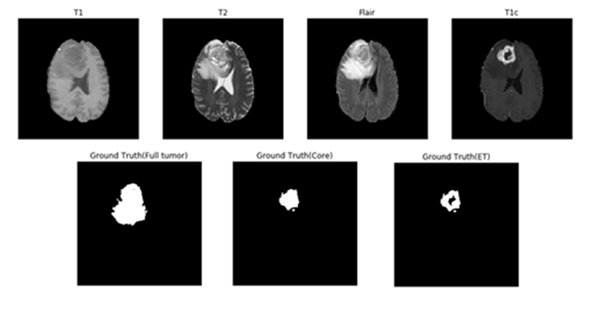
\includegraphics[scale=0.43]{Figures/MRI.png}
      \caption[Dataset Overview]{One axial slice of an MR image of a high-grade glioma patient. From left to right in row 1: T1-weighted image, T2-weighted image, T2-FLAIR-weighted image T1-weighted image with contrast enhancement. In row 2, showing the three sub-region ground truth labeled by exports}
      \label{fig:MRI_slice}
 \end{figure}

%-----------------------------------------------------------------------------------------------------------------------------------------------------------------------------------------------------------------------------------------------------